\documentclass[10pt,t]{beamer} % handout
\usetheme{Heverlee}
\usepackage{amsmath, amssymb}
\usepackage{tikz}
\usepackage{tikz-cd}
\usepackage{mathbbol}

% environments
%\newtheorem{theorem}{Theorem}
%\newtheorem{proposition}[theorem]{Proposition}
%\newtheorem{lemma}[theorem]{Lemma}
%\newtheorem{corollary}[theorem]{Corollary}
%\theoremstyle{definition}
%\newtheorem{definition}[theorem]{Definition}
%\newtheorem{example}[theorem]{Example}
%\newtheorem{remark}[theorem]{Remark}

% hyphenation
\hyphenation{co-chain}

% elements
\newcommand{\id}{\mathsf{id}}
\newcommand{\M}{\cM}
\newcommand{\UM}{{\forget(\M)}}
\newcommand{\SL}{{\M_{sl}}}
\newcommand{\USL}{{\forget(\M_{sl})}}
\newcommand{\Surj}{\cX}
\newcommand{\BE}{\cE}

% sets and spaces
\newcommand{\N}{\mathbb{N}}
\newcommand{\Z}{\mathbb{Z}}
\newcommand{\R}{\mathbb{R}}
\renewcommand{\k}{\Bbbk}
\renewcommand{\S}{\mathbb{S}}
\newcommand{\Ftwo}{{\mathbb{F}_2}}
\newcommand{\Fp}{{\mathbb{F}_p}}
\newcommand{\Cp}{{\mathbb{C}_p}}
\newcommand{\graphs}{\mathfrak{G}}
\newcommand{\gsimplex}{\mathbb{\Delta}}
\newcommand{\gcube}{\mathbb{I}}
\newcommand{\scube}[1]{(\triangle^{\!1})^{\times #1}}

% categories
\newcommand{\Cat}{\mathsf{Cat}}
\newcommand{\Fun}{\mathsf{Fun}}
\newcommand{\Set}{\mathsf{Set}}
\newcommand{\Top}{\mathsf{Top}}
\newcommand{\Ch}{\mathsf{Ch}}
\newcommand{\simplex}{\triangle}
\newcommand{\sSet}{\mathsf{sSet}}
\newcommand{\cube}{\square}
\newcommand{\cSet}{\mathsf{cSet}}
\newcommand{\Alg}{\mathsf{Alg}}
\newcommand{\coAlg}{\mathsf{coAlg}}
\newcommand{\biAlg}{\mathsf{biAlg}}
\newcommand{\sGrp}{\mathsf{sGrp}}
\newcommand{\Nec}{\mathsf{Nec}}
\newcommand{\nSet}{\mathsf{nSet}}
\newcommand{\Mon}{\mathsf{Mon}}
\newcommand{\Smod}{\mathsf{Mod}_{\S}}
\newcommand{\Sbimod}{\mathsf{biMod}_{\S}}
\newcommand{\operads}{\mathsf{Oper}}
\newcommand{\props}{\mathsf{Prop}}

% operators
\DeclareMathOperator{\free}{F}
\DeclareMathOperator{\forget}{U}
\DeclareMathOperator{\yoneda}{\mathcal{Y}}
\DeclareMathOperator{\chains}{N}
\DeclareMathOperator{\schains}{N^{\simplex}}
\DeclareMathOperator{\cchains}{N^{\cube}}
\DeclareMathOperator{\cochains}{N^{\vee}}
\DeclareMathOperator{\scochains}{N^{\vee}_{\simplex}}
\DeclareMathOperator{\ccochains}{N^{\vee}_{\cube}}
\DeclareMathOperator{\gchains}{C}
\DeclareMathOperator{\sSing}{Sing^{\simplex}}
\DeclareMathOperator{\cSing}{Sing^{\cube}}
\DeclareMathOperator{\loops}{\Omega}
\DeclareMathOperator{\cobar}{\mathbf{\Omega}}
\DeclareMathOperator{\triangulate}{\mathcal{T}}
\DeclareMathOperator{\cubify}{\mathcal{U}}
\DeclareMathOperator{\projection}{\pi}
\DeclareMathOperator{\inclusion}{\iota}

% other
\renewcommand{\th}{\mathrm{th}}
\newcommand{\op}{\mathrm{op}}
\DeclareMathOperator*{\colim}{colim}
\DeclareMathOperator{\coker}{coker}
\newcommand{\tensor}{\otimes}
\newcommand{\End}{\mathrm{End}}
\newcommand{\Hom}{\mathrm{Hom}}
\newcommand{\bars}[1]{\lvert#1\rvert}
\newcommand{\norm}[1]{\lVert#1\Vert}
\newcommand{\angles}[1]{\langle#1\rangle}
\newcommand{\pairing}[2]{\langle#1, #2\rangle}
\newcommand{\xla}[1]{\xleftarrow{#1}}
\newcommand{\xra}[1]{\xrightarrow{#1}}
\newcommand{\defeq}{\stackrel{\mathrm{def}}{=}}
\newcommand{\pdfEinfty}{\texorpdfstring{${E_\infty}$}{E-infty}}

% letters
\newcommand{\bC}{\mathbb{C}}

\newcommand{\cA}{\mathcal{A}}
\newcommand{\cB}{\mathcal{B}}
\newcommand{\cC}{\mathcal{C}}
\newcommand{\cD}{\mathcal{D}}
\newcommand{\cE}{\mathcal{E}}
\newcommand{\cM}{\mathcal{M}}
\newcommand{\cN}{\mathcal{N}}
\newcommand{\cO}{\mathcal{O}}
\newcommand{\cP}{\mathcal{P}}
\newcommand{\cW}{\mathcal{W}}
\newcommand{\cX}{\mathcal{X}}
\newcommand{\cY}{\mathcal{Y}}
\newcommand{\cZ}{\mathcal{Z}}

\newcommand{\rB}{\mathrm{B}}
\newcommand{\rE}{\mathrm{E}}
\newcommand{\rP}{\mathrm{P}}
\newcommand{\rR}{\mathrm{R}}

\newcommand{\sA}{\mathsf{A}}
\newcommand{\sB}{\mathsf{B}}
\newcommand{\sC}{\mathsf{C}}

% comments
\newcommand{\anibal}[1]{\textcolor{blue}{\underline{Anibal}: #1}}


\newsavebox\precoproduct
\begin{lrbox}{\precoproduct}
	\begin{tikzpicture}[scale=.3]
	\draw (0,0)--(0,.8);
	\draw (0,0)--(.5,-.5);
	\draw (0,0)--(-.5,-.5);
	\end{tikzpicture}
\end{lrbox}
\newcommand{\coproduct}{% <- this 'right of' is inherited; how to avoid?
	\usebox\precoproduct}

\newsavebox\preproduct
\begin{lrbox}{\preproduct}
	\begin{tikzpicture}[scale=.3]
	\draw (0,0)--(0,-.8);
	\draw (0,0)--(.5,.5);
	\draw (0,0)--(-.5,.5);
	\end{tikzpicture}
\end{lrbox}
\newcommand{\product}{% <- this 'right of' is inherited; how to avoid?
	\usebox\preproduct}

%%% QUICK OPTIONS:
% (A) Math font without serifs, enable line below to make math serif:
    \usefonttheme[onlymath]{serif}

% (B) Re-define primary colour by adjusting the RGB values
    %\definecolor{pblue}	{RGB}{206,125,66}

% (C) Title page graphic (optional) --- this is not for the background image, see \usebackgroundtemplate to change that ---
    %\titlegraphic{\includegraphics[height=2.7cm]{example_figure.pdf}}

% (D) Add logo to bottom right-corner (optional)
    \logo{\includegraphics[height=0.7cm]{icosahedron-src.pdf}\hspace{12pt}\vspace{-6pt}}

% (E) Choose one (or none) of these lines to add footline bar on all frames
    %\setbeamertemplate{footline}[infoline]  % author, title, insitute
    %\setbeamertemplate{footline}[navigation] % dots swhowing progress
    %\setbeamertemplate{footline}[navsym] % navigation symbols

% (F) Widescreen 16:9 ratio
    %\usepackage[orientation=landscape,size=custom,width=16,height=9,scale=0.45,debug]{beamerposter}



%%% TITLE PAGE INFO:

\title[clesto]{Effective construction in algebraic topology and applications}
\author[ammedmar]{Anibal M. Medina-Mardones}
\institute{Max Planck Institute for Mathematics in Bonn}
\date{August 2021}

\begin{document}
{
% Change image, or delete this line to remove background image
\usebackgroundtemplate{ \parbox[b][\paperheight][b]{\paperwidth}{\centering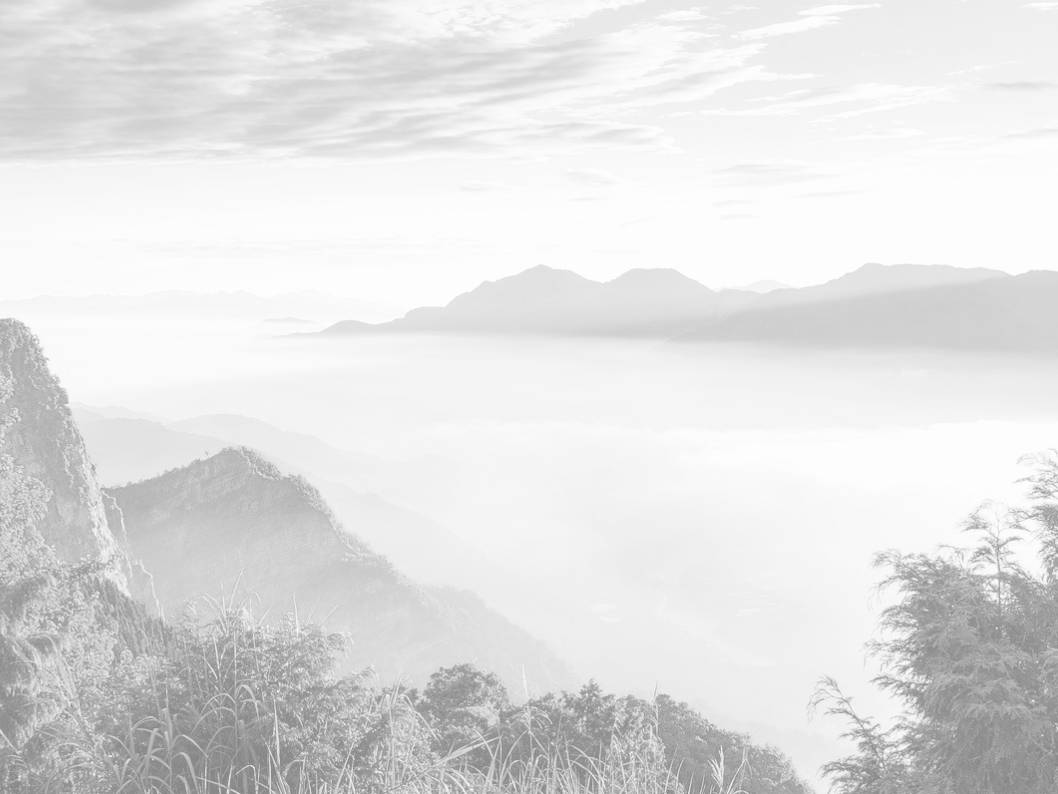
\includegraphics[width=\paperwidth]{bg_alishan.jpg}}}
 %   abudhabi      cherry      forest      river
 %   alishan       chobe       leuven      sanfancisco
 %   blueprint     columns     library     uyuni
 %   bokeh         flowers     newyork     winter

%\setbeamercolor{background canvas}{bg=lgray}  % make background light gray

\begin{frame}[plain,noframenumbering]
    \titlepage
\end{frame}
}

% Table of contents slide
%\begin{frame}{Outline}
%	\vskip 2mm
%	\hfill	{\large \parbox{.95\textwidth}{\tableofcontents[hideothersubsections]}}
%\end{frame}

%\section{History and motivation}

\begin{frame}{Philosophical viewpoint}
	\vskip -10pt
	\begin{block}{Postulate}
		A principal goal of algebraic topology, if not its \textit{raison d'\^{e}tre}, is to encode the theory of topological spaces up to some specified notion of equivalence in terms of combinatorial or algebraic objects, allowing for the quantitative analysis of topological properties.
	\end{block}

	\medskip \pause
	\begin{block}{A basic tension}
		Computability vs. strength of invariants.
	\end{block}

	\medskip \textcolor{pblue}{Example:}
	Homology vs. homotopy.

	\medskip \pause
	\begin{block}{A more subtle tension}
		Effectiveness vs. functoriality of their constructions.
	\end{block}

	\medskip \textcolor{pblue}{Example:}
	cohomology via a cochain complex or \\
	\hspace*{40pt} via maps to Eilenberg-Maclane spaces.
\end{frame}

\begin{frame}{Modeling spaces combinatorially}
	\pause
	\begin{block}{Poincar\'{e}}
		Break spaces into contractible combinatorial pieces: simplices, cubes, ...
	\end{block}

	\pause \textcolor{pblue}{Cohomology:}
	via a cochain complex generated by these pieces.

	\medskip \pause	More generally:
	\begin{block}{Kan-Quillen}
		Use category theory to replace spaces by functors with a geometric realization: simplicial sets, cubical sets, ...
	\end{block}

	\pause \textcolor{pblue}{Basic objects:}
	Chains on standard pieces $\gchains(\gsimplex^n)$, $\gchains(\gcube^n)$, ...

	\smallskip \pause
	\begin{block}{Our goal (loosly stated)}
		Understand this chain complexes deeply to enhance (co)homology with finer effectively computable invariants.
	\end{block}
\end{frame}

\begin{frame}{Shortcomings of (co)homology}
	\pause With mod 2 coefficients the real projective plane and the wedge of a sphere and a circle are isomorphic
	\[
	H^\bullet(\R P^2; \Ftwo) \cong H^\bullet(S^1 \vee S^2; \Ftwo)
	\]
	as graded vector spaces.

	\bigskip \pause
	Similarly,
	\[
	H^\bullet(\mathbb{C} P^2; \Z) \cong H^\bullet(S^2 \vee S^4; \Z)
	\]
	as graded abelian groups.

	\bigskip \pause
	\begin{block}{Cup product}
		These can be distinguished by the algebra/ring structure in cohomology.
	\end{block}
\end{frame}

\begin{frame}[fragile]{$1^{\mathrm{st}}$ example of effect. construct.: cup product}
	\pause Alexander and Whitney defined the cup product by dualizing a chain approximation to the diagonal:
	\[
	\gchains(\gsimplex^n) \to \gchains(\gsimplex^n) \otimes \gchains(\gsimplex^n).
	\]
	\pause Similarly, Cartan and Serre constructed: $\gchains(\gcube^n) \to \gchains(\gcube^n) \otimes \gchains(\gcube^n)$.

	\bigskip \pause
	As mentioned before, as graded rings,
	\[
	H^\bullet(\mathbb{C} P^2) \not\cong H^\bullet(S^2 \vee S^4).
	\]

	\vskip -8pt \pause But,
	\[
	H^\bullet(\Sigma(\mathbb{C} P^2)) \cong H^\bullet(\Sigma(S^2 \vee S^4)),
	\]
	where $\Sigma$ denotes suspension, for example $\Sigma(S^1)$ is
	\begin{center}
		\includegraphics[scale=.2]{aux/suspension.pdf}
	\end{center}
\end{frame}

\begin{frame}{$2^{\mathrm{nd}}$ example of effect. construct.: Steenrod squares}
	\pause These chain approximations, unlike the diagonal of spaces, are \textcolor{pblue}{not} invariant under transposition: $x \otimes y \stackrel{T}{\mapsto} y \otimes x$.

	\medskip \pause By correcting homotopically the breaking of this symmetry, Steenrod defined further structure on mod 2 cohomology:
	\[
	Sq^k \colon H^\bullet(X; \Ftwo) \to H^\bullet(X; \Ftwo).
	\]

	\pause These \textcolor{pblue}{distinguish} $H^\bullet(\Sigma(\mathbb{C} P^2))$ from $H^\bullet(\Sigma(S^2 \vee S^4))$.

	\medskip \pause Steenrod introduced his corrections by effectively constructing
	\[
	\cW(2) \otimes \gchains(\gsimplex^n) \to \gchains(\gsimplex^n) \otimes \gchains(\gsimplex^n),
	\]
	an equivariant chain map where $\cW(2)$ is the minimal free resolution of $\Z$ as an $\Z[\S_2]$-module: $\Z[\S_2]\{e_0\} \xla{1-T} \Z[\S_2]\{e_1\} \xla{1+T} \dotsb$

	\bigskip \pause The map $\Delta_i \colon \gchains(\gsimplex^n) \to \gchains(\gsimplex^n)^{\otimes 2}$ defined by $e_i$ is called \textit{cup-$i$ coproduct}.
\end{frame}

\begin{frame}[fragile]{A new description of Steenrod's construction}
	\pause \vskip -5pt \textcolor{pblue}{Notation:} \vspace*{-5pt}
	\[
	d_u[v_0, \dots, v_m] = [v_0, \dots, \widehat v_u, \dots, v_m]
	\]
	\pause \vspace*{-15pt}
	\[
	\rP_q(n) = \big\{ U \subseteq \{0,\dots,n\} : \bars{U} = q \big\}
	\]
	\pause \vspace*{-15pt}
	\[
	\forall \, U = \{u_1 < \dots < u_q\} \in \rP_q(n)
	\]
	\pause \vspace*{-15pt}
	\[
	d_U = d_{u_1} \dotsm \, d_{u_q}
	\]
	\pause \vspace*{-15pt}
	\[
	U^\varepsilon = \big\{ u_i \in U \mid u_i + i \equiv \varepsilon \text{ mod } 2 \big\}
	\]
	\pause \vskip -10pt
	\begin{definition}[Med.]
		For a basis element $x \in \gchains_m(\gsimplex^n)$
		\vspace*{-5pt}
		\[
		\Delta_i(x) \ = \!\!\! \sum_{U \in \rP_{i-m}(n)} \!\! d_{U^0}(x) \otimes d_{U^1}(x)
		\]
		\vspace*{-10pt}
	\end{definition}
	\pause \textcolor{pblue}{Example:} \vspace*{-5pt}
	\begin{align*}
	\Delta_0 [0,1,2] &=
	\Big( d_{12} \otimes \id + d_2 \otimes d_1 + \id \otimes d_{01} \Big) [0,1,2]^{\otimes 2} \\ &=
	[0] \otimes [0,1,2] + [0,1] \otimes [1,2] + [0,1,2] \otimes [2].
	\end{align*}
\end{frame}

\begin{frame}{The relevance of cochain level Steenrod squares}
	\pause \vskip -5pt \textcolor{pblue}{Cup-$i$ (co)products:} \smallskip
	\begin{enumerate}
		\item Are used in the definition of action functionals for lattice models in topological quantum field theory (Gaiotto, Kapustin, Thorngren, ...) \pause
		\item Are used in persistence homology to extract finer information of data sets (Lupo--Med.--Tauzin) \pause
		\item Can used to construct effective chain approximations to spin bordism (Brumfiel--Morgan) \pause
		\item Can be used to construct cochains enforcing the Cartan relation (Med.) and Adem relation (Brumfiel--Med.--Morgan) \pause
		\item Can be axiomatically characterized in analogy to the axioms for Steenrod square (Med.) \pause
		\item Define the nerve of higher categories (Med.) \pause
		\item Are used to construct mod-2 operations on Khovanov homology (Cantero-Mor\'{a}n) \pause
		\item \ $\cdots$
	\end{enumerate}
\end{frame}

\begin{frame}{Operations at odd primes}

	Steenrod also defined operations
	\[
	\beta^{\varepsilon} P_k \colon H^\bullet(X; \Fp) \to H^\bullet(X; \Fp).
	\]

	\pause How to generalize the cup-$i$ products to cochain level operations for all $p$?

	\smallskip \pause
	\begin{enumerate}
		\item Construct $\S_p$-equivariant chain maps
		\[
		\rE \S_p \otimes \gchains \to \gchains^{\otimes p}
		\]
		for $\rE \S_p$ a resolution of $\Z$ by free $\Z[\S_p]$-modules.
		\vspace*{10pt} \pause
		\item Identify chains in $\rE \S_p$ whose orbits in $(\rE \S_p)_{\S_p} = \rB \S_p$ represent mod-$p$ homology classes.
	\end{enumerate}

	\medskip \pause	The first step is systematized using the theory of \textit{operads}.

	\smallskip \pause The second uses that $\bC_p \to \S_p$ induces a surjection in mop-$p$ homology.
\end{frame}

\begin{frame}[fragile]{Canonical example of operad}
	\pause Let $C$ be a chain complex, consider the set
	\[
	\End^C = \left\{ \Hom(C, C^{\otimes r}) \right\}_{r \geq 1}.
	\]

	\pause	Ii is equipped with the structure of an operad:
	\begin{enumerate}
		\item A left action of $\S_r$ on $\End^C(r)$, \pause
		\item Composition chain maps
		\[
		\begin{tikzcd}[column sep=small, row sep=tiny]
		\circ_i \colon &[-10pt] \End^C(r) \otimes \End^C(s) \arrow[r] & \End^C(r+s-1) \\
		& f \otimes g \arrow[r, |->] & (1 \otimes \cdots \otimes g \otimes \cdots \otimes 1) \circ f
		\end{tikzcd}
		\]
	\end{enumerate}
	satisfying forms of equivariance, associativity, and unitality.

	\pause \vspace*{10pt}

	\textcolor{pblue}{Slogan:} Abstract groups are to automorphism groups like operads are to these coendomorphism operads.
\end{frame}

\begin{frame}{A graphical example}
	\pause Consider the directed labeled graph
	\[
	\begin{tikzpicture}[scale=.5]
	\draw (0,0)--(0,.75);
	\draw (0,0)--(.5,-.5);
	\draw (0,0)--(-.5,-.5);
	\node[scale=.5] at (-.5,-.75){1};
	\node[scale=.5] at (.5,-.75){2};
	\end{tikzpicture}
	\]

	\pause Define $\cA(r)$ to be the free module generated by all (relabeled) ``graftings"
	\[
	\begin{tikzpicture}[scale=.75]
	\draw (-.5,1)--(.5,1)--(.5,0)--(-.5,0)--(-.5,1);
	\node[scale=.75] at (0,.5){$\Gamma$};

	\draw (0,1)--(0,1.25);
	\node[scale=.5] at (0,1.5){1};

	\draw (-.5,0)--(-.5,-.25);
	\node[scale=.5] at (-.5,-.5){1};
	\draw (.5,0)--(.5,-.25);
	\node[scale=.75] at (.5,-.5){$r$};
	\node[scale=.75] at (0,-.5){$\cdots$};
	\end{tikzpicture}
	\quad
	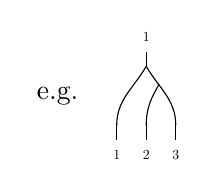
\begin{tikzpicture}[scale=.75]

	\node at (-1.5, 0.5){e.g.};
	\draw (0,1)--(0,1.25);
	\node[scale=.5] at (0,1.5){1};

	\draw (0,1) to  [out=-120,in=90] (-.5,0);
	\draw (0,1) to  [out=-60,in=90] (.5, 0);
	\draw (.22,.7) to  [out=-120,in=90] (0,0);

	\draw (-.5,0)--(-.5,-.25);
	\node[scale=.5] at (-.5,-.5){1};
	\draw (0,0)--(0,-.25);
	\node[scale=.5] at (0,-.5){2};
	\draw (.5,0)--(.5,-.25);
	\node[scale=.5] at (.5,-.5){3};
	\end{tikzpicture}
	\vspace*{-5pt}
	\]

	\medskip \pause An operad morphism $\cA \to \Hom^C$ is determined by the assignment
	\[
	\coproduct \mapsto \Delta
	\]
	of an element $\Delta \in \Hom(C, C^{\otimes 2})$, i.e., of a coalgebra structure on $C$.
\end{frame}

\begin{frame}[fragile]{\pdfEinfty-coalgebras}
	Let $\cO$ be an operad, a $\cO$-\textit{coalgebra} on $C$ is a structure preserving
	\[
	\cO \to \End^C.
	\]
	\pause This corresponds to compatible equivariant maps $\cO(r) \otimes C \to C^{\otimes r}$.

	\medskip \pause	Compare with Steenrod's	\vspace*{-5pt}
	\[
	\begin{tikzcd}[%
	row sep=tiny,
	column sep = small,
	,row sep = 0ex
	,/tikz/column 1/.append style={anchor=base east}
	,/tikz/column 2/.append style={anchor=base west}
	]
	\cW(2) \arrow[r] & \Hom \left( \gchains, \gchains^{\otimes 2} \right) \\
	e_i \arrow[r, |->] & \Delta_i
	\end{tikzcd}
	\]

	\pause \vspace*{-10pt}
	\begin{definition}
		An operad $\cO$ is said to be $E_\infty$ if each $\cO(r)$ is a free resolution of $\Z$ by $\Z[\S_r]$-modules
	\end{definition}

	\smallskip \pause Coalgebras over $E_\infty$-operads are thought of as being coassociative and cocommutative up to coherent homotopies.
\end{frame}

\begin{frame}{A finitely presented model}
	\pause Consider the directed labeled graphs
	\[
	\begin{tikzpicture}[scale=.5]
	\draw (0,0)--(0,.75);
	\draw (0,0)--(.5,-.5);
	\draw (0,0)--(-.5,-.5);
	\node[scale=.5] at (-.5,-.75){1};
	\node[scale=.5] at (.5,-.75){2};
	\end{tikzpicture}
	\qquad
	\begin{tikzpicture}[scale=.5]
	\draw (0,0)--(0,-.75);
	\draw (0,0)--(.5,.5);
	\draw (0,0)--(-.5,.5);
	\node[scale=.5] at (-.5,.75){1};
	\node[scale=.5] at (.5,.75){2};
	\end{tikzpicture}
	\vspace*{-10pt}
	\]

	Define $\M(s, r)_n$ as the free module generated by all (relabeled) ``graftings" and disjoint unions of these of the form
	\[
	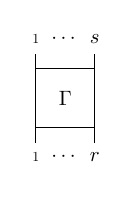
\begin{tikzpicture}[scale=.75]
	\draw (-.5,1)--(.5,1)--(.5,0)--(-.5,0)--(-.5,1);
	\node[scale=.75] at (0,.5){$\Gamma$};

	\draw (-.5,1)--(-.5,1.25);
	\node[scale=.5] at (-.5,1.5){1};
	\draw (.5,1)--(.5,1.25);
	\node[scale=.75] at (.5,1.5){$s$};
	\node[scale=.75] at (0,1.5){$\cdots$};

	\draw (-.5,0)--(-.5,-.25);
	\node[scale=.5] at (-.5,-.5){1};
	\draw (.5,0)--(.5,-.25);
	\node[scale=.75] at (.5,-.5){$r$};
	\node[scale=.75] at (0,-.5){$\cdots$};
	\end{tikzpicture}
	\vspace*{-5pt}
	\]
	with $n$-copies of the \product.
	\pause The boundary map is obtained by removing their incoming strands one at the time: \vspace*{-5pt}
	\[
	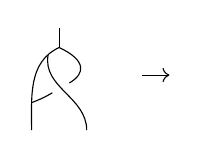
\begin{tikzpicture}[scale=.35]
	\draw (1,3.7) to (1,3);
	\draw (1,3) to [out=205, in=90] (0,0);
	\draw [shorten >= 0cm] (.6,2.73) to [out=-100, in=90] (2,0);
	\draw [shorten >= .15cm] (1,3) to [out=-25, in=30, distance=1.1cm] (1,1.5);
	\draw [shorten <= .1cm] (1,1.5) to [out=210, in=20] (0,1);

	\draw[->] (4,2) to (5,2);
	\end{tikzpicture}
	\qquad %%%%%%%%%%
	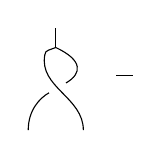
\begin{tikzpicture}[scale=.35]
	\draw (1,3.7) to (1,3);
	\draw (1,3) to [out=205, in=90] (.6,2.73);
	\draw [shorten >= 0cm] (.6,2.73) to [out=-100, in=90] (2,0);
	\draw [shorten >= .15cm] (1,3) to [out=-25, in=30, distance=1.1cm] (1,1.5);
	\draw [shorten <= .1cm] (1,1.5) to [out=210, in=90] (0,0);

	\draw (3.2,2) to (3.8,2);
	\end{tikzpicture}
	\quad %%%%%%%%%%
	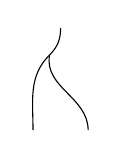
\begin{tikzpicture}[scale=.35]
	\draw (1,3.7) to [out=-90, in=45] (.6,2.73);
	\draw (.6,2.73) to [out=225, in=90] (0,0);
	\draw [shorten >= 0cm] (.6,2.73) to [out=-100, in=90] (2,0);
	\end{tikzpicture}
	\]
\end{frame}

\begin{frame}{A finitely presented model}
	\begin{theorem}[Med.]
		The operad $\UM$ defined by $\UM(r) = \M(1,r)$ is $E_\infty$.
	\end{theorem}

	\pause Furthermore, the assignments
	\[
	\coproduct \mapsto \Delta
	\qquad
	\product \mapsto \ast
	\vspace*{-10pt}
	\]
	where
	\[
	\Delta \colon \gchains(\gsimplex^n) \to \gchains(\gsimplex^n)^{\otimes 2}, \qquad
	\ast \colon \gchains(\gsimplex^n)^{\otimes 2} \to \gchains(\gsimplex^n)
	\]
	 are the AW coproduct and the algebraic join, \pause
	 and in the cubical case the CS coproduct and a suitable analogue, induce the following.
	\pause
	\begin{theorem}[Med.]
		The complexes $\gchains(\gsimplex^n)$ and $\gchains(\gcube^n)$ are natural $\UM$-coalgebras.
	\end{theorem}
	\pause
	We remark that explicitly describable elements in $\UM(2)$ recover the Steenrod cup-$i$ coproducts in the simplicial and cubical case.
\end{frame}

\begin{frame}[fragile]{May-Steenrod structures}
	\vskip -5pt \pause The data needed to define the cochain level Steenrod operations is a
	$\bC$-equivariant quasi-isomorphism $\cW \to \UM$ where $\cW(r)$ is the minimal free resolution: $\Z[\bC_r]\{e_0\} \xla{} \Z[\bC_r]\{e_1\} \xla{} \dotsb$

	\medskip \pause Using the explicit contraction of $\UM$ we built such map effectively,
	referring to the image of $e_i \in \cW(r)$ as the cup-$(r,i)$ coproduct.

	\medskip \pause For example, $\Delta_{3,2}[0,1,2]$ is equal (using \verb|ComCh|) to

	\begin{center}
		\begin{verbatim}
		- [0,1][0,1,2][0,1] + [0,1,2][0,2][0,1] + [0,2][0,2][0,1,2]
		- [0,1,2][0,1,2][1] - [0,2][0,1,2][1,2] + [0,1,2][1,2][1,2]
		- [0,1][1,2][0,1,2] - [0,1,2][2][0,1,2] - [0][0,1,2][0,1,2]
		\end{verbatim}
	\end{center}

	\pause \textcolor{pblue}{Future directions:} \pause
	\begin{enumerate}
		\item Where are these used in physics? \pause \\
		\item Faster implementations for use in TDA. \pause \\
		\item Steenrod operations in Khovanov homology. \pause \\
		\item Cartan and Adem coboundaries. \pause \\
		\item Relation to higher category theory.
	\end{enumerate}
\end{frame}

\end{document}


\section{Chain level Steenrod operations for spaces}

\begin{frame}[fragile]{Steenrod $(r,i)$-coproducts on spaces}
	Now that we have preferred cycles in $\M(p)$ representing the mod-$p$ homology of $\S_p$, how do we choose maps $\gchains \to \gchains^{\otimes p}$ for them?
	\[
	\begin{tikzcd}[column sep=small, row sep=tiny]
	r = 2 \ \colon &[-10pt] e_i \arrow[r, |->] & \Delta_i \\
	r > 2 \ \colon & e_i \arrow[r, |->] & ?
	\end{tikzcd}
	\]

	\pause

	We just say where the generators go:
	\[
	\begin{tikzcd}[row sep = small]
	& \mathrm{Simplicial} & \mathrm{Cubical} \\
	\begin{tikzpicture}[scale=.75]
	\draw (0,.5)--(0,1.25);
	\draw (0,.5)--(.5,0);
	\draw (0,.5)--(-.5,0);
	\end{tikzpicture}
	& \begin{tikzpicture}
	\draw[color=pblue, thick] (0,0)--(1,1);
	\draw[->] (1.25, .5) -- (1.75, .5);
	\end{tikzpicture}
	\begin{tikzpicture}
	\node at (-0.1, 1){};
	\draw[color=pblue, thick] (0,0)--(1,0)--(1,1);
	\draw (1,1)--(0,1)--(0,0);
	\end{tikzpicture}
	& \begin{tikzpicture}
	\draw[color=pblue, thick] (0,0)--(1,1);
	\draw[->] (1.25, .5) -- (1.75, .5);
	\end{tikzpicture}
	\begin{tikzpicture}
	\node at (-0.1, 1){};
	\draw[color=pblue, thick] (0,0)--(1,0)--(1,1);
	\draw (1,1)--(0,1)--(0,0);
	\end{tikzpicture} \\
	\begin{tikzpicture}[scale=.75]
	\draw (0,.75)--(0,0);
	\draw (0,.75)--(.5,1.25);
	\draw (0,.75)--(-.5,1.25);
	\end{tikzpicture}
	& \begin{tikzpicture}
	\draw (0,0)--(1,0)--(1,1)--(0,0);
	\draw[->] (1.25, .5) -- (1.75, .5);
	\filldraw[fill=pblue, draw=pblue] (0,0) circle (1pt);
	\filldraw[fill=pblue, draw=pblue] (1,1) circle (1pt);
	\end{tikzpicture}
	\begin{tikzpicture}
	\node at (-0.1, 1){};
	\draw[color=pblue, thick] (0,0)--(1,1);
	\draw (1,1)--(1,0)--(0,0);
	\end{tikzpicture}
	& \begin{tikzpicture}
	\draw (0,0)--(0,1)--(1,1)--(1,0)--(0,0);
	\draw[->] (1.25, .5) -- (1.75, .5);
	\filldraw[fill=pblue, draw=pblue] (0,0) circle (1pt);
	\filldraw[fill=pblue, draw=pblue] (1,1) circle (1pt);
	\end{tikzpicture}
	\begin{tikzpicture}
	\node at (-0.1, 1){};
	\draw[color=pblue, thick] (0,0)--(0,1)--(1,1);
	\draw (1,1)--(1,0)--(0,0);
	\end{tikzpicture}
	\end{tikzcd}
	\]
\end{frame}

\begin{frame}{Steenrod $(r,i)$-coproducts on spaces}

	For example: \vspace*{-20pt}
	\begin{center}
	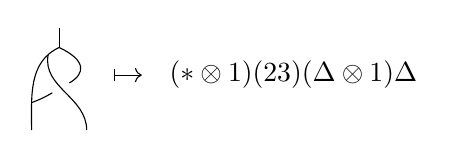
\begin{tikzpicture}[scale=.35]
	\draw (1,3.7) to (1,3);
	\draw (1,3) to [out=205, in=90] (0,0);
	\draw [shorten >= 0cm] (.6,2.73) to [out=-100, in=90] (2,0);
	\draw [shorten >= .15cm] (1,3) to [out=-25, in=30, distance=1.1cm] (1,1.5);
	\draw [shorten <= .1cm] (1,1.5) to [out=210, in=20] (0,1);

	\draw[|->] (3,2) to (4,2);

	\node at (9.5,2){$(\ast \otimes 1)(23)(\Delta \otimes 1)\Delta$};
	\end{tikzpicture}
	\end{center}

	\pause

	It turns out that the image of $e_i$ in $\M(r)$ is in the linear span of
	\begin{center}
		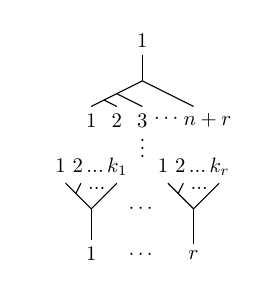
\begin{tikzpicture}[scale=.65]
		\draw (0,0)--(0,-.6) node[below, scale=.75]{$1$};
		\draw (0,0)--(.5,.5);
		\draw (-.3, .3)-- (-.2,.5) node[above, scale=.75]{\quad $1\ 2\, ...\, k_1$};
		\draw (-.5,.5)--(0,0);
		\node[scale=.75] at (.11,.4){$...$};

		\node[scale=.75] at (1,0){$\cdots$};
		\node[scale=.75] at (1,-.9){$\cdots$};

		\draw (2,0)--(2,-.68) node[scale=.75, below]{$r$};
		\draw (2,0)--(2.5,.5);
		\draw (1.7, .3)-- (1.8,.5) node[scale=.75, above]{\quad $1\ 2\, ...\, k_r$};
		\draw (1.5,.5)--(2,0);
		\node[scale=.75] at (2.11,.4){$...$};

		\draw (1,2.5)--(1,3) node[scale=.75, above]{$1$};
		\draw (1,2.5)--(0,2) node[scale=.75, below]{$1$};
		\draw (.25,2.125)--(.5,2) node[scale=.75, below]{$2$};
		\draw (.5,2.25)--(1,2) node[scale=.75, below]{$3$};
		\draw (1,2.5)--(2,2) node[scale=.75, below]{\ \quad $n + r$};
		\node[scale=.75] at (1.5,1.75){$\cdots$};

		\node[scale=.75] at (1,1.3) {$\vdots$};

		\node at (2.85,0){};
		\end{tikzpicture}
	\end{center}
	which can be described by surjections $s \colon \{1, \dots, r+n\} \to \{1, \dots, r\}$.

	\pause \vspace*{10pt}

	\textcolor{pblue}{Comment (not used today)} The surjection operad is a quotient of $\M$.
\end{frame}


\begin{frame}{Explicit examples}
	Image of $e_i$ in $\M(r)$ for small values of $r$ and $i$. \vspace*{-10pt}
	\begin{table}[h]
		\centering
		\resizebox{\columnwidth}{!}{%
			\renewcommand{\arraystretch}{1.3}
			\begin{tabular}{|c||c|c|c|}
				\hline
				$r$& $n=2$ & $n=3$ & $n=4$ \\
				\hline
				2 & (1,2,1,2) & (1,2,1,2,1) & (1,2,1,2,1,2) \\
				\hline
				3 & (1,2,3,1,2) + (1,3,1,2,3) & (1,2,3,1,2,3) + (1,2,1,2,3,1)  & \phantom{+} (1,2,3,1,2,3,1) + (1,2,3,2,3,1,2) \\
				& + (1,2,3,2,3) & + (1,2,3,1,3,1) & + (1,2,3,1,2,1,2) + (1,3,1,2,3,1,2) \\
				& & & + (1,3,1,3,1,2,3) + (1,2,3,2,3,2,3) \\
				& & & + (1,3,1,2,3,2,3) \\
				\hline
				4 & \phantom{+} (1,2,3,4,1,2) + (1,3,4,1,2,3) & \phantom{+} (1,2,3,4,1,2,3) + (1,2,4,1,2,3,4) & \\
				& + (1,2,3,4,2,3) + (1,4,1,2,3,4) & + (1,2,3,4,1,3,4) + (1,2,1,2,3,4,1) & 25 \text{ terms } \\
				& + (1,2,4,2,3,4) + (1,2,3,4,3,4) & + (1,2,3,1,3,4,1) + (1,2,3,4,1,4,1) & \\
				\hline
			\end{tabular}
		}
	\end{table}

	\pause

	Passing from the Steenrod $(p,i)$-coproducts to Steenrod operations on the mod-$p$ cohomology of spaces, we have two families indexed by integers:
	\[
	P_s, \beta P_s \colon H^\bullet(-;\F_p) \to H^\bullet(-;\F_p).
	\]

	\pause

	Hyperlink to interactive examples:

	\vspace*{5pt}
	\qquad \href{https://comch.readthedocs.io/en/latest/}{\beamergotobutton{ComCH}}

	\vspace*{0pt}
	\qquad \href{https://mybinder.org/v2/gh/ammedmar/comch/master?filepath=notebooks\%2Fsteenrod_operations.ipynb}{\beamergotobutton{Steenrod}}

\end{frame}

\section*{References}

\begin{frame}[allowframebreaks]
	\frametitle{References}
	\nocite{whitney1935history}
	\nocite{steenrod47products}
	\nocite{brumfiel2018pontrjagin}
	\nocite{brumfiel2020cochain}
	\nocite{cantero2020khovanov}
	\nocite{medina2018axiomatic}
	\nocite{medina2018persistence}
	\nocite{medina2020prop1}
	\nocite{medina2018prop2}
	\nocite{medina2020globular}
	\nocite{medina2020cartan}
	\nocite{medina2020odd}
	\bibliographystyle{amsalpha}
	\bibliography{biblio.bib}
\end{frame}


\end{document}
